\FloatBarrier
\Needspace{14\baselineskip}
\section{Efficiency and Power Difference}
\label{sec:res-efficiency}

Output power, initial efficiency, and input--output power difference
were calculated as
\begin{align}
P_\mathrm{out}&=V_\mathrm{BUS,avg}I_\mathrm{out},
\label{eq:pout-from-vbus-iout}\\
\eta&=\frac{P_\mathrm{out}}{P_\mathrm{in}}\,100\%,
\label{eq:efficiency}\\
P_\mathrm{difference}&=P_\mathrm{in}-P_\mathrm{out}.
\end{align}
Average VBUS and external load current were used to calculate output power,
with analyzer readings for input power. The resulting efficiency estimates
are preliminary because simultaneous acquisition and the inclusion of all
auxiliary power paths are not fully documented.

\begin{figure}[htbp]
\centering
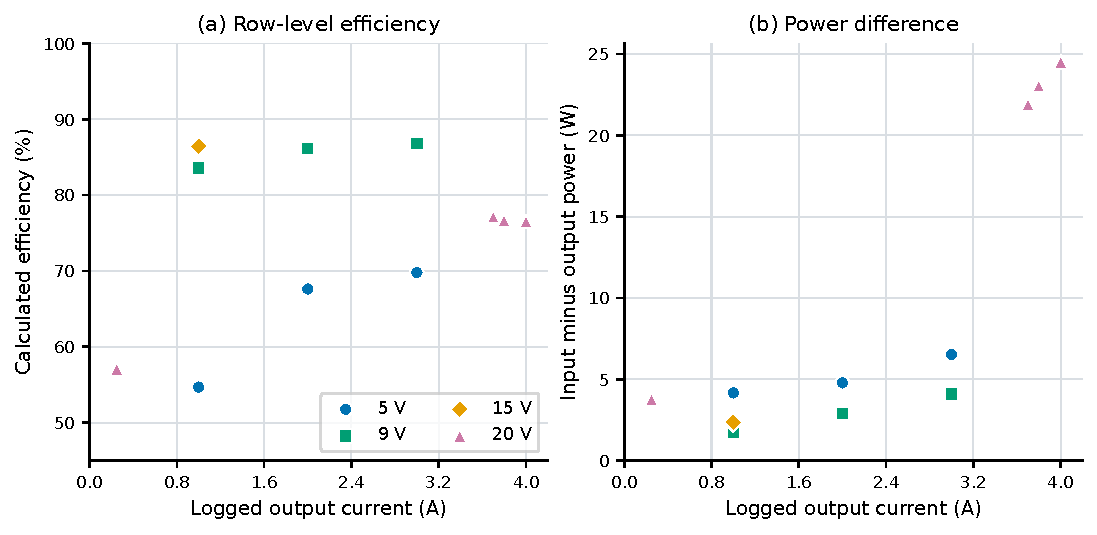
\includegraphics[width=\textwidth]{Pictures/Thesis/10_Results/Rebuilt/efficiency_and_loss.pdf}
\caption{Initial efficiency estimates and input-minus-output power from eleven tests. Marker shapes identify the fixed output voltage. }
\label{fig:rebuilt-efficiency-loss}
\end{figure}

At \SI{5}{\volt}, the calculated value rises from about
\SI{54.7}{\percent} at \SI{1}{\ampere} to \SI{69.8}{\percent} at
\SI{3}{\ampere}. The \SI{9}{\volt} points range from
\SI{83.6}{\percent} to \SI{86.8}{\percent}, the highest of the eleven
selected rows. The \SI{15}{\volt}, \SI{1}{\ampere} result is
\SI{86.4}{\percent}. The tests used different instruments and operating histories, so these
values do not form a calibrated efficiency map.

\Needspace{20\baselineskip}
% Automatically rebuilt from original records by rebuild_results.py.
\begingroup
\scriptsize
\setlength{\tabcolsep}{3pt}
\renewcommand{\arraystretch}{1.12}
\begin{longtable}{@{}L{0.3022\linewidth} L{0.1067\linewidth} L{0.1244\linewidth} L{0.1244\linewidth} L{0.0978\linewidth} L{0.1244\linewidth}@{}}
\caption{Initial efficiency estimates from eleven measurements.}\label{tab:efficiency-results}\\
\toprule
Test ID & $I_\mathrm{out}$ (A) & $P_\mathrm{out}$ (W) & $P_\mathrm{in}$ (W) & $\eta$ (\%) & Difference (W)\\
\midrule
\endfirsthead
\toprule
Test ID & $I_\mathrm{out}$ (A) & $P_\mathrm{out}$ (W) & $P_\mathrm{in}$ (W) & $\eta$ (\%) & Difference (W)\\
\midrule
\endhead
\sourcefile{PDO5-5W-001} & 1.00 & 5.03 & 9.20 & 54.69 & 4.17\\
\sourcefile{PDO5-10W-2A-001} & 2.00 & 9.99 & 14.78 & 67.61 & 4.79\\
\sourcefile{PDO5-MAX3A-001} & 3.00 & 15.06 & 21.59 & 69.79 & 6.52\\
\sourcefile{PDO20-5W-001} & 0.25 & 5.01 & 8.78 & 57.09 & 3.77\\
\sourcefile{PDO20-75W-001} & 3.70 & 73.97 & 95.88 & 77.15 & 21.91\\
\sourcefile{PDO20-76W-38A-001} & 3.80 & 75.93 & 98.99 & 76.70 & 23.06\\
\sourcefile{PDO20-80W-40A-001} & 4.00 & 79.89 & 104.42 & 76.51 & 24.53\\
\sourcefile{PDO9-9W-1A-001} & 1.00 & 9.02 & 10.80 & 83.56 & 1.77\\
\sourcefile{PDO9-18W-2A-001} & 2.00 & 18.03 & 20.93 & 86.14 & 2.90\\
\sourcefile{PDO9-27W-3A-001} & 3.00 & 27.00 & 31.10 & 86.82 & 4.10\\
\sourcefile{PDO15-15W-1A-001} & 1.00 & 15.01 & 17.37 & 86.41 & 2.36\\
\bottomrule
\end{longtable}
\endgroup


The \SI{20}{\volt} high-power tests give \SI{77.15}{\percent},
\SI{76.70}{\percent}, and \SI{76.51}{\percent} at
\SI{3.7}{\ampere}, \SI{3.8}{\ampere}, and \SI{4.0}{\ampere}.
Their input--output differences are \SI{21.91}{\watt},
\SI{23.06}{\watt}, and \SI{24.53}{\watt}. At \SI{4}{\ampere},
\SI{104.418}{\watt} logged input accompanies \SI{79.8928}{\watt}
calculated output. The total difference does not allocate loss among the GaN
stage, inductors, charge pump, output interface, and auxiliary supply;
intermediate-stage power measurements are required.

No-load, transient, and AC-coupled output rows were excluded, along with the
\SI{3.9}{\ampere}, \SI{20}{\volt} row with an associated input capture
and the \SI{15}{\volt}, \SI{2}{\ampere} and \SI{3}{\ampere} rows
whose notes flag real-power disagreement. Siglent/ITECH disagreement remains in several selected groups; the selected
workbook entries are used consistently, but the instrument error remains unresolved.
A matched sweep must synchronize settled input/output readings and account
for auxiliaries, cable drop, temperature, and propagated uncertainty.
